\chapter{Defining finite entailment sets}
\label{chap:entailments}
The justificatory structure of an OWL ontology \O describes the relationships between the justifications for \emph{some} set of entailments of \O. However, if we want to compute the set of justifications for \enquote{the entailments} of an ontology, we immediately encounter a problem: recall that the set of entailments of an ontology \O is the set of all axioms \axiom such that \O \entails \axiom---a set which is infinite for OWL ontologies, and in most cases it does not seem practical to compute and analyse justifications (other than the empty ontology over a non-empty signature) for an infinite set of entailments. 

Thus, we need to restrict the set of entailments we analyse to some \emph{finite} subset of the deductive closure of \O. Classification of an ontology, that is, computing all entailed subsumptions and equivalences containing only named classes, is a standard reasoning task, and the resulting class hierarchy (in the form of either the atomic subsumption axioms or both subsumption and equivalence axioms) of the ontology is a commonly used entailment set in OWL applications.

However, even if we restrict our attention to the class hierarchy of an ontology, we find that there is no standard way of \emph{representing} this set of axioms. Worse even, misleading nomenclature in ontology tools, such as the \protege editor and the OWL API, as well as anecdotal evidence show that there exist common misconceptions about the entailments: it is often assumed that only non-trivial information is contained in the set of entailments, and tautologies such as \dlax{A \subcls A} are not \enquote{real} entailments. On the other hand, however, some OWL tools \emph{do} include tautologies of the type \dlax{A \subcls \thing} for certain named classes. And finally, the term \enquote{entailments} is frequently used to refer to information which is only \emph{inferred} but not asserted in the ontology, leading to asserted axioms not being considered entailments.

This means that, despite having a well-defined finite set of entailments at hand (the set of all axioms $\alpha$ of type \dlax{A \subcls B} and, if required, \dlax{A \eqcls B} for $A, B \in \sig{\O}$ such that $\O \models \alpha$), we still obtain different numbers of entailments for the same ontology depending on the representation chosen by the application we are dealing with. And while it may not be necessary to define a single canonical representation of the class hierarchy---after all, axioms such as \dlax{A \subcls \thing} \emph{can} be useful for some applications while they might be superfluous in others---we need to at least make obvious the different design decisions to be made when choosing a representation for this entailment set.

In what follows, we will discuss various design decisions for representing finite entailment sets  of consistent OWL ontologies, which takes into consideration relationships such as direct and indirect subsumptions, tautologies, dealing with unsatisfiable and universal classes, and ontology imports, while paying attention to the issue of \emph{counting} entailments. The design decisions presented here largely focus on the class hierarchy of an ontology, but are also applicable to arbitrary entailments, and we will also discuss how we can define finite entailment sets \emph{beyond} the simple class hierarchy of an ontology. Finally, we introduce a shorthand notation which allows us to conveniently refer to a specific representation of an entailment set, and outline some examples of how entailment sets are used in OWL applications. 

While this chapter informs the experiments on justifications presented in the remainder of this thesis, it may also be regarded as a self-standing discussion with relevance to applications such as ontology analysis, the OWL API, and ontology editing tools.


\section{Design decisions for finite entailment sets}

In this section, we will describe a number of design decisions to make when choosing a representation for a finite entailment set of an OWL ontology. In other words, given a finite set of entailments, such as the axioms representing the class hierarchy, we suggest a set of filtering steps which result in an axiom set that is logically equivalent, but may differ in the number of axioms it contains.

To clarify the distinction between a finite entailment set and its representation, consider a simple example: given an ontology \O = $\{A \subcls B, B \subcls C\}$, we are interested in all entailed atomic subsumptions of type \dlax{X \subcls Y} where $X \not= Y$, $X \not= \nothing$, and $Y \not= \thing$. This gives us the finite entailment set \entset = $\{A \subcls B, B \subcls C, A \subcls C\}$. However, we may also choose to \emph{represent} \entset by an equivalent, more compact set of axioms \entset' = $\{A \subcls B, B \subcls C\}$, which is logically equivalent to \entset, but contains fewer axioms. 

Only the choice of entailment types has an effect on the actual \emph{size} of a finite entailment set: given two ontologies \O and \oprime such that $\O \subset \oprime$, we expect the number of axioms in a finite entailment set of the \emph{larger} ontology \oprime to be the same or more than that of \O. That is, our notion of finite entailment sets must be \emph{stable} under the extension of an ontology \O; an essential criterion when using entailment counts for the comparison of two ontologies. 

However, as we will see in the following sections, some design decisions for \emph{representations} of entailment sets appear to violate the stability of the entailment set relation by leading to \emph{smaller} (representations of) entailment sets when \emph{adding} axioms to an ontology. Where applicable, we will point out the impact of a decision on the stability of entailment counts.


\subsection{Tautologies}
A tautology is an axiom such as \dlax{A \subcls A}, \dlax{A \subcls \thing}, and \dlax{\nothing \subcls A} for a named class \dlcn{A \in \sig{\O}} which is vacuously entailed by \O. Tautologies do not contain any relevant information and are therefore frequently omitted from the axiom set representing the class hierarchy of an ontology.

However, in some OWL tools, such as the OWL API and \protege, named classes that do not have a direct named subsumer are generally \emph{included} in entailment sets as subclasses of \thing, in order to ensure that all named classes in the ontology are present in the entailment set in some way. Note that this strategy means that \emph{only} classes which do not have a named subsumer occur in axioms of the type \dlax{A \subcls \thing}. This can be problematic if we use the entailment count to compare the logical strength of two ontologies: take, for instance, two ontologies over the signature $\{A, B, C\}$ where \O = $\emptyset$ and $\oprime = \{A \subcls B\}$. If we include axioms of the above type in the entailment set, we get the two entailment sets 
\begin{align*}
\varepsilon_{\O} =& \{ \dlax{A \subcls \thing}, \dlax{B \subcls \thing}, \dlax{C \subcls \thing}\}\\
\varepsilon_{\oprime} =& \{\dlax{A \subcls B}, \dlax{B \subcls \thing}, \dlax{C \subcls \thing}\}.
\end{align*}
Both entailment sets have the same number of entailments; however, $\varepsilon_{\oprime}$ arguably contains at least \emph{some} non-trivial information (namely the subsumption \dlax{A \subcls B}). While this decision does not affect the monotonicity of the entailment count, it shows that, if we include tautologies in an entailment set, the size of the set may not reflect the amount of relevant information it contains.

Since there is no obvious benefit to including most tautologies in a finite entailment set, we will generally consider finite entailment sets to be free of tautologies in the remainder of this chapter. If required, we may only include axioms of the type \dlax{A \subcls \thing} for a named class \dlcn{A} which does not have any other named subsumer. 


\subsection{Asserted and inferred axioms}

Every axiom that is asserted in an ontology \O is trivially entailed by the ontology and therefore part of the set of entailments of \O. However, the main idea behind logic-based ontologies is the application of automated reasoning to make \emph{implicit} knowledge visible; thus, the set of \emph{inferred}, but not asserted, axioms may be of much higher relevance to a user. In particular when counting entailments of an ontology, including asserted axioms in the count may not add any useful information if the number of asserted axioms of the selected type is already known. Most OWL tools (e.g.\ \protege and the OWL API) take this into account when representing the class hierarchy of an ontology and return only entailments which are inferred, but not asserted.

While excluding asserted axioms from an entailment set is a reasonable choice in user-focused applications, this may lead to a loss of information in analytical applications, such as justification analysis. An entailment that is asserted in an ontology may also hold for other, more complex reasons, i.e.\ it can have justifications other than the asserted axiom itself. This may be purely accidental and a side-effect of other axioms in the ontology, or intentional as a result of ontology developers \enquote{adding} inferred entailments into the ontology. Making entailments explicit has two advantages: first, it may improve reasoner performance when classifying the ontology, as the reasoner will have to perform fewer subsumption checks, and second, the information will be visible even when there is no reasoner available, for example in a web-based ontology browser---and even if these are not real benefits, users may \emph{believe} that they are, which encourages them to take these steps. 

When counting entailments, we need to be aware of the effects of excluding asserted entailments from the entailment set. Assume an ontology \O with $n$ asserted atomic subsumptions and $k \geq 1$ inferred (but not asserted) atomic subsumptions. If we only count entailments which are inferred but not asserted, the entailment count for \O will be $k$. Now, if we add all $k$ inferred atomic subsumption axioms to \O, we obtain \oprime such that $\O \subset \oprime$. Then the entailment set of \oprime will contain no (inferred but not asserted) axioms, that is, $\varepsilon_{\oprime} \subset \varepsilon_{\O}$ despite $\O \subset \oprime$. This is obviously counter-intuitive, as we generally expect the number of entailments to grow monotonically as we add axioms to an ontology. 

A more concrete example shows how the distinction between inferred and asserted entailment makes the entailment count dependent on the syntactical variations of equivalent axioms: take $\O = \{\dlax{A \subcls B \conj C}\}$ and $\oprime = \{\dlax{A \subcls B}, \dlax{A \subcls C}\}$. \O has two entailed atomic subsumptions (\dlax{A \subcls B}, \dlax{A \subcls C}) which are inferred and not asserted, whereas \oprime, despite having the same entailed atomic subsumptions, has no entailments according to our specification.

Of course, in both examples the \enquote{missing} entailments are only a deception, as the two ontologies are logically equivalent, which means they do not actually differ in terms of their information content; however, if we use that the number of inferred (and not asserted) entailments as an ontology metric to compare the two ontologies, we can easily see how this situation can quickly lead to counting errors.


\subsection{Transitivity}

We generally treat the class hierarchy of an ontology as a directed graph, with nodes representing sets of equivalent classes, and edges representing subsumption relationships. A \emph{direct} subsumption between a class \dlcn{A} and a class \dlcn{B} is represented by an edge between the nodes labelled with \dlcn{A} and \dlcn{B}, respectively; this corresponds to a path of size one. An \emph{indirect} subsumption is a path between two nodes of size greater than one. The class graph can be either based on the \emph{asserted} ontology, i.e.\ the class graph is constructed based on the axioms in the ontology, without the use of a reasoner, or the \emph{inferred} ontology, which means that the class graph is built according to the subsumptions and equivalences returned by a reasoner. That is, a directed edge between the nodes labelled \dlcn{A} and \dlcn{B} is added to the class graph of \O if \dlax{A \subcls B} is asserted in (inferred by) \O, and a class name \dlcn{C} is added to the label of a node labelled $\{D\}$ if \dlax{C \eqcls D} is asserted in (inferred by) \O. Note that in \protege, the class hierarchy display is generated using a very simple \emph{structural} reasoner which, in addition to implementing transitivity of the subsumption relationship, simply splits conjunctions on the RHS of subsumption axioms and in equivalent classes axioms.

The set of all entailed atomic subsumptions, direct and indirect, then corresponds to the transitive \emph{closure} of the inferred class graph, while the transitive \emph{reduct} \cite{aho72pz} represents the set of entailed \emph{direct} subsumptions. The transitive reduct of a directed acyclic graph $G$ is a graph $G'$ such that $G'$ has a directed path between two nodes $u,v$ whenever there is a path ($u, v$) in $G$, and there is no graph with fewer edges than $G'$ which fulfils that condition. The abstract concept of a transitive reduct can be represented as the Hasse diagram\footnote{See, for example, \cite{joslyn06aa} for an example of diagrammatic representations of an OWL ontology.} of an ontology's class graph.

There are several scenarios in which we may want to include or exclude indirect subsumptions in a representation of the class hierarchy. When presenting a set of entailed axioms to a user, we may  assume that the user understands the principle of transitivity and only requires a small entailment set with \emph{relevant} information; in such a case, it seems reasonable to choose a compact representation of the entailment set by excluding indirect subsumptions. On the other hand, if a user wants to be presented with \emph{all} the information entailed by an ontology, it might be preferable to include indirect subsumptions. For the purpose of computing and analysing justifications of an ontology, for example, we may want to include indirect subsumptions in the entailment set, as they may have relevant justifications which would otherwise be neglected.

With regards to counting the number of entailments of an ontology, care needs to be taken when dealing with the transitive reduct of the inferred class graph. Example \ref{ex:transreductontology} shows how \emph{removing} axioms from an ontology results in an \emph{increase} in the number of entailments.
\begin{examp}\begin{align*}
		\O = \{&\dlax{X_{1}  \subcls A}, \dlax{X_{2}  \subcls A}, \dlax{X_{3}  \subcls A}\\
		&\ax{X_{1}  \subcls B}, \dlax{X_{2}  \subcls B}, \dlax{X_{3}  \subcls B}, \dlax{A \subcls B} \}\end{align*}\label{ex:transreductontology}\end{examp}
Given the above ontology, the number of entailed direct atomic subsumptions, based on the transitive reduct of the inferred class graph (shown in Figure \ref{fig:inf-classgraph-before}), is 4, as the indirect subsumptions between \dlcn{X_{i}} and \dlcn{B} are excluded from the set: $\entset = \{\dlax{X_{1}  \subcls A},  \dlax{X_{2}  \subcls A}, \dlax{X_{3}  \subcls A}, \dlax{A  \subcls B} \!\:\}$. Removing the axiom \dlcn{A \subcls B} from the ontology creates the class graph for the now modified ontology \oprime shown in Figure \ref{fig:inf-classgraph-after}; as we can see, the transitive reduct of the graph has \emph{more} edges than the graph for \O. Accordingly, the set of entailments based on the transitive reduct now contains 6 entailed axioms: $\varepsilon_{\oprime} = \{\dlax{X_{1}  \subcls A},  \dlax{X_{2}  \subcls A}, \dlax{X_{3}  \subcls A}, \dlax{X_{1}  \subcls B},  \dlax{X_{2}  \subcls B}, \dlax{X_{3}  \subcls B}\!\:\}$. Thus, the removal of an axiom has led to a seemingly \emph{larger} entailment set in this particular representation.

\begin{figure}
\centering
		\begin{subfigure}{0.5\textwidth}
                \centering
                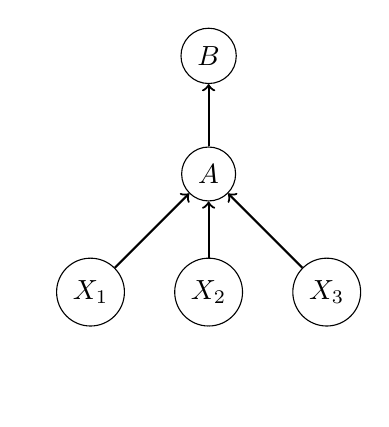
\begin{tikzpicture}
\tikzstyle{every node}=[draw,shape=circle];

  \node (b) at (1.5,3) {$B $};
  \node (a) at (1.5,1.5) {$A$};
    
  \node (x1) at (0,0) {$X_{1}$};
  \node (x2) at (1.5,0) {$X_{2}$};
  \node (x3) at (3,0) {$X_{3}$};
\foreach \from/\to in {a/b, x1/a, x2/a, x3/a}
\draw [->,thick] (\from) -- (\to);
    
    
\draw[->,line width=0.5pt, color=white]  (x2.south) to [out=-90,in=-90]  ([xshift={-10}]x1.west) to [out=90,in=-180] (b.west);

\end{tikzpicture}


                \caption{Transitive reduct of \O.}
        	\label{fig:inf-classgraph-before}
        \end{subfigure}%
        ~ %add desired spacing between images, e. g. ~, \quad, \qquad etc.\ 
          %(or a blank line to force the subfigure onto a new line)
		\begin{subfigure}{0.5\textwidth}
                \centering
                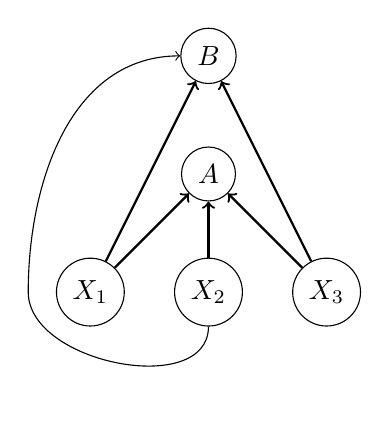
\begin{tikzpicture}
\tikzstyle{every node}=[draw,shape=circle];

  \node (b) at (1.5,3) {$B$};
  \node (a) at (1.5,1.5) {$A$};
    
  \node (x1) at (0,0) {$X_{1}$};
  \node (x2) at (1.5,0) {$X_{2}$};
  \node (x3) at (3,0) {$X_{3}$};
\foreach \from/\to in { x1/a, x2/a, x3/a,x1/b, x3/b}
\draw [->,thick] (\from) -- (\to);


\draw[->] (x2.south) to [out=-90,in=-90]  ([xshift={-10}]x1.west) to [out=90,in=-180] (b.west);
    
\end{tikzpicture}


                \caption{Transitive reduct of \oprime.}
        	\label{fig:inf-classgraph-after}
        \end{subfigure}
\end{figure}

Interestingly, the \texttt{InferredSubClassAxiomGenerator} implemented by the OWL API exhibits exactly this behaviour; and while this non-monotonicity of entailment counts may be technically correct, it is certainly confusing and counter-intuitive to a user who has no way of specifying and understanding the exact settings of an entailment generator.

\subsection{Equivalent classes}
\label{sec:repfunction}

While we commonly only deal with entailed atomic subsumptions representing the class hierarchy, we might also want to include information about the equivalence between named classes in the ontology in an entailment set. However, dealing with equivalent classes (or properties) axioms as entailments is not as straightforward as it may seem, as choosing how to represent equivalent classes as well as subsumptions between equivalent classes and other classes as a set of axioms requires us to make a number of design decisions.

\paragraph{Representing equivalence as axioms}

Assume some ontology \O entails the equivalence of the classes \dlcn{A}, \dlcn{B}, and \dlcn{C}. In the class graph of \O this can be easily expressed by a node which is labelled with the three class names. In OWL applications, however, users are generally presented with a list of entailed \emph{axioms} rather than a graph visualisation. We now have to choose how to represent the equivalence between these three classes in a set of equivalent classes axioms: 
\begin{compactenum}
\item As an n-ary \dlcn{EquivalentClasses} axiom, which is possible in OWL.
\item As an exhaustive set of binary equivalent classes axioms in order to correspond to DL notation which only allows binary equivalent classes axioms
\item As a minimal set of binary equivalent classes axioms. This requires the use of a function $Pairwise(n)$ to return a set of \emph{pairwise} axioms which suffices to represent the relation, such as $\{\dlax{A \eqcls B}, \dlax{B \eqcls C}\}$. This method is implemented in the OWL API.
\end{compactenum}

Again, the decision how to represent equivalent classes depends on the application of the entailment set. In an OWL context, an n-ary \ax{EquivalentClasses} axiom is certainly the most user-friendly way of representing a set of equivalent classes. When analysing justifications, an exhaustive set of binary equivalent class axioms will capture all justifications, while a set of representative axioms may be suitable in a user-facing application which only supports binary equivalent classes axioms.

\paragraph{Subsumptions between equivalent classes}
Representing the subsumption relationships in a class graph between nodes labelled with multiple equivalent classes poses yet another challenge: given a set of equivalent classes \dlcn{A}, \dlcn{B}, and \dlcn{C} which are all subsumed by a common superclass \dlcn{D}, how can we represent this relation in a set of axioms? 

Yet again, there are multiple approaches, which depend on whether an entailment set explicitly contains equivalence classes axioms, or whether the equivalence between (sets of) classes may be represented otherwise:
\begin{compactenum}

\item Every class in the set of equivalent classes creates a new subsumption axiom \dlax{A \subcls D}, \dlax{B \subcls D}, \dlax{C \subcls D}. If the chosen entailment set does \emph{not} include equivalent class axioms, this approach may be suitable, as it explicitly lists the subsumption relations between all classes and their superclasses.\footnote{Excluding the equivalent class axioms in this situation may lead a user to have an incorrect  \enquote{mental model} of the ontology graph in which the three subclasses are not equivalent.} The disadvantage of this strategy is a fast growth of subsumption axioms if both the subclass and the superclass node contain multiple equivalent classes. That is, for two nodes labelled with $i$ and $j$ equivalent classes, respectively, the number of axioms resulting from this approach is $i*j$.
 
\item When including equivalent class axioms in the entailment set, it may suffice to select a \emph{representative} from each of the nodes representing the sub- and superclasses, respectively. For this purpose, we introduce a new function, $Rep(n)$ which selects a class name from a node $n$ of equivalent classes based on some user-defined criteria. The knowledge of the equivalence relations and the subsumption between two of the classes will then be sufficient information for a user to infer that the other subsumptions follow. 

\item Another, less straightforward approach, would be to attempt to represent all equivalent classes in a node by one newly generated class name, for example by concatenating the names of the subclasses and presenting the user an axiom of the type \dlax{A, B, C \subcls D}. This is obviously not standard OWL notation and might be confusing to a user, yet, it conveniently captures both the equivalence as well as the subsumption relations in a single axiom.

\end{compactenum}


\subsection{Strict and non-strict subsumptions}

Another issue to consider when computing finite entailment sets is the notion of representing strict vs non-strict subsumptions. A strict subsumption is an axiom \dlax{A \subcls B} such that \dlax{\O \entails A \subcls B} and \dlax{\O \not\entails B \subcls A}, i.e.\ the classes are not equivalent, whereas a non-strict subsumption is an axiom \dlax{A' \subcls B'} or \dlax{B' \subcls A'}  where \dlax{\O \entails A' \eqcls B'}. 

By default, OWL reasoners (when accessed via the OWL API) exclude non-strict subsumptions when asking for all superclasses of a named class. This may cause confusion in cases where a user knows that class \dlcn{A} should be subsumed by \dlcn{B}, but is not aware of reasons for the equivalence of the two classes; the subsumption simply appears to be missing from the entailment set. Including non-strict subsumptions therefore seems reasonable when a user requests only subsumption axioms and no equivalent classes axioms in an entailment set. On the other hand, when including equivalence  axioms in an entailment set, non-strict subsumptions should in turn be excluded from the set in order to avoid duplicating information in the resulting set.

When counting entailments, we are faced with yet another situation in which the number of entailments does not grow monotonically in the size of the ontology. Take the two ontologies $\O = \{\dlax{A \subcls B}\}$ and $\oprime = \{\dlax{A \subcls B}, \dlax{B \subcls A}\}$. \oprime clearly contains more axioms and is stronger than \O, however, if we count only strict subsumptions in the entailment set (as is the default in the OWL API), the number of entailments of \oprime is less than that of \O. As in the previous examples, the \emph{actual} number of entailments of \oprime as given by the entailment relation \entails is greater than that of \O, however, our entailment sets \emph{appear} to violate the monotonicity of \entails.

\subsection{Equivalence to top and bottom}

An unsatisfiable class in an ontology is a class which is equivalent to \nothing, i.e.\ it is mapped to the empty set in all interpretations. This also means that any unsatisfiable class is a subclass of any other class in the ontology. In ontology editors and in conversational use, however, unsatisfiable classes are frequently denoted as \emph{subclasses of bottom} and no subsumptions between the unsatisfiable class and named classes are included in entailment sets. For example, the OWL API's \texttt{InferredSubClassOfAxiomGenerator} only returns atomic subsumptions involving \emph{satisfiable} classes.

Similarly, a class which is entailed to be equivalent to \thing (we may call it a \emph{tautological} class) is commonly denoted as \emph{superclass of \thing}, and is entailed to be a superclass of any other named class in the ontology. Interestingly, there is no symmetry between the treatment of unsatisfiable and tautological classes, as entailments of the type \dlax{B \subcls A} for a tautological class \dlax{A \eqcls \thing} and a named class $B$ \emph{are} commonly displayed in ontology editors and returned by the OWL API. 

Regarding the naming conventions, while these are obviously not incorrect, they only show one direction of the equivalence relationship between the classes which may be misleading to users; furthermore, if we exclude non-strict subsumptions from an entailment set in a principled manner, we should also exclude axioms of the type \dlax{A \subcls \nothing} and \dlax{\thing \subcls A}, as these are non-strict subsumptions. On the other hand, for both \thing and \nothing the subsumption in one direction (\dlax{\nothing \subcls A}, \dlax{A \subcls \thing}) is in fact trivial, and we are really only interested in the other direction of the equivalence. This is why it seems reasonable to treat equivalences with \thing and \nothing separately from named classes and generally display them as subsumption axioms.

With respect to the different treatment of unsatisfiable and tautological classes, it is clear to see that a tautological class can introduce more subtle errors in the ontology, while subsumptions involving unsatisfiable classes do not contain any relevant information. Take, for instance, the \emph{Movie} ontology example which we have mentioned in Chapter 2. In this ontology, the class \cn{Person} is entailed to be unsatisfiable. This is caused by the fact that the class \cn{Movie} is tautological (i.e.\ \enquote{everything is a \cn{Movie}}), but asserted to be disjoint with \cn{Person}. Understanding that \cn{Movie} is a superclass of \cn{Person} is crucial to understanding the cause of the error. This example shows how (direct or indirect) subsumptions involving tautological classes add important information to an entailment set and should therefore always be included in an entailment set.


\subsection{Axiom and expression types}


Thus far we have focused on the design decisions which affect the representation of the class hierarchy of an ontology. However, it is clear to see that an application might require a finite entailment set which contains axiom and expression types beyond atomic subsumptions and equivalences. For example, it can be useful to know how many named classes are subsumed by an expression such as \dlax{\exists r.B} for an arbitrary named property $r$ and class $B$, as this can justify the introduction of a named class for the anonymous expression. This means that we need some way of restricting the infinite set of entailments of an OWL ontology to a sensible finite set, which strikes a balance between containing large amounts of irrelevant information and omitting relevant axioms.

\emph{Prime implicates} \cite{quine52aa,quine59aa,jackson92aa,bienvenu09aa} fulfil the requirement of providing a finite representation of the set of entailments of a formula. Initially defined for propositional formulae, Bienvenu \cite{bienvenu07aa} extends the notion of prime implicates to concept expressions in the description logic \dl{ALC}. First, literals $L$, clauses $Cl$, and cubal concepts $Cb$ are defined as follows:
\begin{align*}
L ::=  &\thing \mid \nothing \mid A \mid \neg A \mid \forall r.Cl \mid \exists r.Cb \\
Cl ::= & L \mid Cl \sqcup Cl \\
Cb ::= & L \mid Cb \sqcap Cb
\end{align*}
A clausal concept $Cl$ is then a prime implicate of a concept expression $C$ if 
\begin{compactenum}
\item $\models C \sqsubseteq Cl$
\item For any $Cl'$ such that $\models Cl' \sqsubseteq Cl$, then $\models Cl \sqsubseteq Cl'$.
\end{compactenum}

Prime implicates are the \enquote{logically strongest clausal consequences} \cite{bienvenu09aa} of a formula that do not contain any redundancies; removing any literal from a prime implicate would cause the clause to no longer be entailed. Prime implicates of this type do not correspond to our notion of entailments as sets of axioms, but rather describe subsumptions between expressions. We can obtain a finite set of axioms, for example, by generating the set of class assertions $x:Cl$ for all $x:C$, or the set of subsumption axioms $X \subcls Cl$ for all $X \subcls C$ for $x, X \in \sig{O}$. As an example \cite{bienvenu07aa}, take the following expression:
\begin{align*}
A \conj (B \disj C) \conj \exists r.\thing \conj \forall r.(B \conj (A \disj C)) \conj \forall r.(B \disj D)
\end{align*}
The prime implicates of this expression are the expressions $A, B \disj C, \exists r.(B \conj A) \disj \exists r.(B \conj C), \forall r.B, \forall r.(A \disj C)$.

While prime implicates provide an elegant way of defining a \enquote{natural} finite set of entailments, the concept has only been extended to concept expressions in \dl{ALC} and does not cover the full spectrum of constructors and axioms available in OWL. We therefore look at simpler, purely syntactical strategies for generating finite entailment sets.

Similar to restricting the finite entailment set to entailed atomic subsumptions, we can specify any other axiom type as well as expression types we want to consider by providing an entailment pattern. In order to generate entailed axioms of different types containing only named classes, the OWL API provides an \texttt{InferredAxiomGenerator} interface whose implementations provide access to generators for \emph{all} OWL axiom types, such as \texttt{InferredDisjointAxiomGenerator} and \texttt{InferredSubDataPropertyAxiomGenerator}.

Beyond atomic entailments, we may also want to include entailments involving \emph{complex} expressions, such as existential or universal quantifiers. Entailments containing complex expressions are currently not supported \enquote{out-of-the-box} by tools such as the OWL API; however, it is certainly possible to programmatically generate axioms containing complex expressions over the signature of an ontology \O, check whether these are entailed by \O, and if yes, include them in the entailment set. 

In order to guarantee that the entailment set generated that way is indeed finite, we need to impose restrictions on the types and nesting depths of expressions. For example, we may only include axioms which do not contain any nested expressions, such as \dlax{A \subcls \exists r.B}, \dlax{A \subcls \forall r.B}, \dlax{A \subcls B \conj C}, \dlax{A \subcls B \disj C}, \dlax{A \subcls \neg B}. Finally, once these complex entailments have been specified, the design decisions we have discussed thus far can be applied in order to choose a suitable representation of the set.



\subsection{Dealing with ontology imports}

Another issue that needs to be dealt with when extracting and counting entailments from an ontology is its import structure. An OWL ontology \O  that imports another OWL ontology \oprime can have different kinds of entailments: those that hold in \O $\setminus$ \oprime (\emph{native} entailments),  those that are entirely from the imported ontology, i.e.\ they hold in  \oprime $\setminus$ \O (\emph{imported} entailments), and those that are neither native, nor imported, and hold in \O $\cup$ \oprime (\emph{mixed} entailments). 

When performing analytical tasks on a corpus of ontologies, disregarding the issue of imported entailments may in fact lead to significant distortions: imagine a scenario where each ontology $\O_{i}$ in a test corpus imports another ontology \oprime, for instance an upper-level ontology. A finite entailment set of each of $\O_{i}$ would also include all imported entailments of \oprime, which would skew any analysis of the corpus towards the entailments of \oprime. We encountered this situation when analysing a snapshot of the NCBO BioPortal\footnote{\url{http://bioportal.bioontology.org/}} corpus, in which a number of ontologies had exactly the same set of entailments, as they were all importing the \emph{Basic Formal Ontology}\footnote{\url{http://www.ifomis.org/bfo}} (BFO).

In order to resolve this issue, we propose a classification of entailment types based on the \emph{origin} of an entailment which is determined by the set of its justifications. We use the following naming conventions:\footnote{As used in \url{http://www.w3.org/TR/owl2-syntax/\#Imports}}

\begin{compactitem}
\item $\O_{root}$ denotes the ontology \emph{document} we are analysing, e.g.\ the .owl file that has been loaded into an ontology editor.
\item \O is the \emph{import closure} of $\O_{root}$, i.e.\ the ontology resulting from transitive closure of the imports of $\O_{root}$.
\item \oprime denotes an ontology in the import closure of $\O_{root}$ that is not the root ontology itself.
\end{compactitem}

Intuitively, a native entailment originates entirely from the root ontology, that is, all its justifications contain only axioms from the root $\O_{root}$. An imported entailment originates entirely from entailments that are \emph{not} from the root ontology, whereas a \emph{mixed} entailment covers the remaining scenarios:

\begin{defn}
A justification \J for an entailment \ent is a
\begin{compactenum}
\item \emph{native} justification in \O if $\J \in \O_{root}$. 
\item \emph{imported} justification in \O if $\J \cap \O_{root} = \emptyset$. 
\item \emph{mixed} justification otherwise.
\end{compactenum}
An entailment \ent is called 
\begin{compactenum}
\item \emph{native} if it has \emph{only} native justifications.
\item \emph{imported} if it has \emph{only} imported justifications.
\item \emph{mixed} otherwise.
\end{compactenum}
\end{defn}

We can see straight away that there are several constellations of mixed entailments having native, imported, and mixed justifications. While such a fine-grained distinction may not be relevant for analytical purposes (it seems more reasonable to simply include \emph{all} entailments of a specified type from an ontology \O and its imports closure), we list them here for completeness:
\begin{compactenum}
\item Purely mixed: An entailment which has \emph{only} mixed justifications.
\item Partially mixed: An entailment which has
\begin{compactenum}[a)]
\item native and imported justifications.
\item mixed and native justifications.
\item mixed and imported justifications.
\item mixed, native, and imported justifications.
\end{compactenum}
\end{compactenum}

\section{A notation for finite entailment sets}

Based on the design decisions we have discussed in the previous section, we will now introduce a shorthand notation for the various aspects of finite entailment sets. The notation will allow us to conveniently refer to specific entailment sets, for example, in OWL tools, the OWL API, and in experiment descriptions. Further, we will also introduce notations for \emph{wanted} and \emph{unwanted} entailment sets to denote partitions of a given finite entailment set. The section is concluded by several examples of entailment sets to demonstrate how the notation we have introduced can be applied in practice.

\subsection{Introducing the notation}


Table \ref{tab:entailmentnotation} lists the keys and polarities (+ or -) we assign to the individual design decisions and the defaults. Note the following remarks:
\begin{compactenum}
\item The keys for the properties in the top section of the table are constructed to always assume the \emph{negative} polarity key as the default where applicable, e.g.\ $T^{-}$. The negative polarity is given simply for completeness reasons and to specify the default; if clear from the context, we choose to simply drop the key to assume the default option.
\item 1. implies that when \emph{including} a certain type of entailment, the + sign indicating positive polarity of the key is not necessarily required; e.g.\ we could simply write $T$ to indicate the presence of \dlax{A \subcls \thing} type axioms. However, we choose to always include the polarities in order to make the decision explicit and avoid ambiguity.
\item The exception with regards to polarity is the inclusion of native entailments by default, indicated by the positive  key $I^{n+} $.
\item Keys and polarities can be grouped, e.g.\ to describe the set of atomic subsumptions including asserted axioms and indirect subsumptions, we write \enquote{the $(AD)^{+}$ set of axioms of the type \dlax{A \subcls B} for all named, satisfiable classes \dlcn{A}, \dlcn{B} in \O}.
\item The decision whether to include unsatisfiable and tautological classes as subsumption or equivalent classes  axioms is omitted from the table, as it is part of the description of the axiom and expression types in an entailment set specification.
\item The keys $E^{r}$ and $N^{r}$ require the specification of a function $Pairwise$ and $Rep$, respectively.
\end{compactenum}

\begin{table}
\caption{Entailment set properties and keys}
\label{tab:entailmentnotation}
\centering
\begin{tabular}{lcc}
\toprule 
Design decision & Keys & Default\\ 
\midrule
Include / exclude axioms of type \dlax{A \subcls \thing} & $T^{+}$ / $T^{-}$ & $T^{-}$\\ 
Include / exclude asserted axioms & $A^{+}$ / $A^{-}$  & $A^{-}$ \\ 
Include / exclude indirect subsumptions & $D^{+}$ / $D^{-}$ & $D^{-}$ \\ 
Include / exclude non-strict subsumptions & $S^{+}$ / $S^{-}$ & $S^{-}$ \\ 
\hline
Representation of equivalent classes & & \\
\midrule
N-ary equivalent classes axioms & $E^{n}$ & $\checkmark$ \\
Exhaustive binary equivalent classes axioms & $E^{e}$ & --  \\
Select pairwise representatives & $E^{r}$ &  -- \\
\midrule
Subsumptions between equivalent classes & & \\
\midrule
Exhaustive subsumption axioms & $N^{e}$ & $\checkmark$ \\
Select representative classes & $N^{r}$ &  -- \\
Introduce new name & $N^{n}$ & -- \\
\midrule
Import types & & \\
\midrule
Include / exclude native entailments & $I^{n+} $/  $I^{n-} $ & $I^{n+}$ \\
Include / exclude imported entailments & $I^{i+}$ / $I^{i-}$ & $I^{i-}$ \\
Include / exclude mixed entailments & $I^{m+}$ / $I^{m-}$  &  $I^{m-}$ \\
\bottomrule
\end{tabular}
\end{table}


\subsection{Axioms and expressions}
Since the range of possible OWL axiom types and expressions to include in the entailment set is very broad, these will not be represented by a key, but described by listing the axiom pattern or expression pattern instead. For example, the set of entailed atomic subsumptions can be described as \enquote{axioms of the type \dlax{A \subcls B} for all named, satisfiable classes \dlcn{A}, \dlcn{B} in \O}. Likewise, we refer to the set of entailed unsatisfiabilities as  \enquote{axioms of the type \dlax{A \subcls \nothing} for all named classes \dlcn{A} in \O}. This can be easily extended to complex expressions, such as \enquote{axioms of the type \dlax{A \subcls \exists r.B} for all named, satisfiable classes \dlcn{A}, \dlcn{B} and named properties \dlcn{r} in \O}.


\subsection{Wanted and unwanted entailments}
\label{sec:wantedunwanted}
In the context of debugging an ontology we usually speak of modifying or removing axioms in order to remove  \emph{unwanted} entailments from the ontology. One of the main concerns here is to find a modification, i.e.\ a repair, such that all unwanted entailments are removed, but at the same time as few \emph{wanted} entailments as possible are lost from the ontology. In the most extreme case, a user could simply remove all axioms from an ontology, which would obviously have the desired effect of removing the unwanted entailments, but at the same time this would also remove any relevant information from the ontology. Borrowing some notation from existing work on revising knowledge bases \cite{shchekotykhin12aa,nikitina12aa}, we introduce names for the sets of wanted and unwanted entailments of an ontology: Given a finite entailment set $\entset = \entsetplus \cup \entsetminus$
\begin{compactitem}
\item \entsetplus is the set of \emph{wanted} entailments
\item \entsetminus  is the set of \emph{unwanted} entailments.
\end{compactitem}

The decision as to which entailments are unwanted lies with the user; a common choice for \entsetminus is the set of entailed subsumption axioms of the type \dlax{A \subcls \nothing} for named classes \dlcn{A} of an ontology. Given these two sets, we can make a clear distinction between modifications which lead to a positive effect (the removal of entailments in \entsetminus) and those with a negative effect (the loss of entailments in \entsetplus). Finding a balance between such positive and negative effects is key in the ontology debugging process; a detailed discussion of this issue will follow in Section \ref{sec:arity}.


\subsection{Sample entailment sets}

The following examples demonstrate the different criteria and their effects on the size and types of axioms of finite entailment sets for a small ontology.

\begin{examp}[Toy ontology \O]
\begin{align*}
&\ax{NorthAmericanCougar\subcls Cougar} &&\ax{Mammal \subcls Animal}\\
&\ax{Cougar \eqcls MountainLion} &&\ax{Puma \eqcls Cougar} \\
&\ax{Puma \subcls Cat} &&\ax{Cat \subcls Mammal}\\
\end{align*}
\end{examp}

The inferred and asserted class graphs of this ontology are shown in Figures \ref{fig:asserted} and \ref{fig:inferred}, respectively.


\begin{figure}
\centering
		\begin{subfigure}{0.4\textwidth}
                \centering
                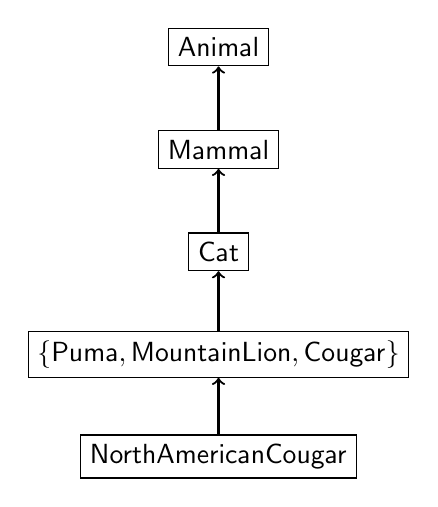
\begin{tikzpicture}
\tikzstyle{every node}=[draw];

  \node (e) at (0,5.2) {$\mathsf{Animal}$};
  \node (d) at (0,3.9) {$\mathsf{Mammal}$};
  \node (c) at (0,2.6) {$\mathsf{Cat}$};
  \node (b) at (0,1.3) {$\mathsf{\{Puma, MountainLion, Cougar\}}$};
  \node (a) at (0,0) {$\mathsf{NorthAmericanCougar}$};
  
  \foreach \from/\to in {a/b, b/c, c/d, d/e}
\draw [->,thick] (\from) -- (\to);
    
    

\end{tikzpicture}


                \caption{Asserted class graph.}
        	\label{fig:asserted}
        \end{subfigure}%
        ~ %add desired spacing between images, e. g. ~, \quad, \qquad etc.\ 
          %(or a blank line to force the subfigure onto a new line)
		\begin{subfigure}{0.6\textwidth}
                \centering
                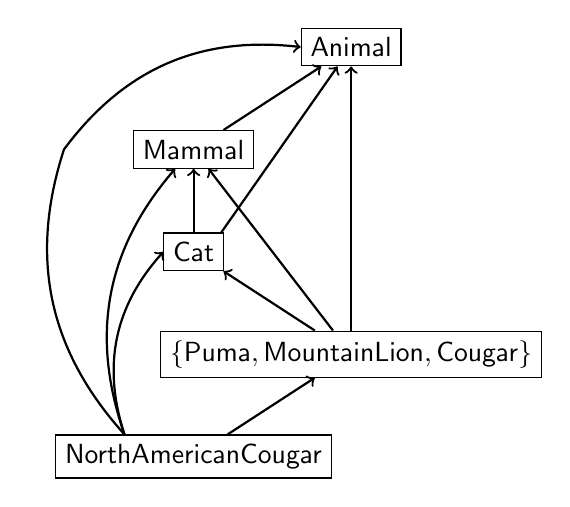
\begin{tikzpicture}
\tikzstyle{every node}=[draw];

  \node (e) at (2,5.2) {$\mathsf{Animal}$};
  \node (d) at (0,3.9) {$\mathsf{Mammal}$};
  \node (c) at (0,2.6) {$\mathsf{Cat}$};
  \node (b) at (2,1.3) {$\mathsf{\{Puma, MountainLion, Cougar\}}$};
  \node (a) at (0,0) {$\mathsf{NorthAmericanCougar}$};
  
  \foreach \from/\to in {a/b, b/c, c/d, d/e, b/d, b/e}
\draw [->,thick] (\from) -- (\to);
    
   \draw [->, bend left,thick] ([xshift={-25}]a.north) to (c.west);
   \draw [->, bend left,thick] ([xshift={-25}]a.north) to (d);
   \draw [->, bend left,thick] ([xshift={-25}]a.north) to ([xshift={-25}]d.west) to (e.west);

   \draw [->, thick] ([xshift={10}]c.north) to (e);
     

\end{tikzpicture}


                \caption{Inferred class graph.}
        	\label{fig:inferred}
        \end{subfigure}
\end{figure}


\paragraph{Transitive closure}

The $(AD)^{+}E^{e}$ entailment set containing axioms of the type \dlax{A \subcls B} and \dlax{A \eqcls B} for satisfiable classes \dlcn{A}, \dlcn{B} in \sig{\O}, make explicit the subsumption and equivalence relationships between every single class in the ontology. The set shown in Example \ref{ex:18ax} is the largest finite entailment set to be extracted from the class graph which does not contain any tautologies. The alternative variant $D^{+}(EN)^{e}$ of this set excluding asserted subsumption axioms simply discards the six axioms that occur in the original ontology, yielding a set of 12 axioms.

\begin{examp}[$(AD)^{+}(EN)^{e}$ entailment set of \O, 18 axioms]
\begin{align*}
& \ax{Cougar \eqcls MountainLion}&&\ax{Cougar \eqcls Puma} \\
& \ax{MountainLion \eqcls Puma} && \ax{Puma \subcls Cat} \\
& \ax{Puma \subcls Mammal} &&\ax{Puma \subcls Animal}\\
& \ax{MountainLion \subcls Cat} &&\ax{MountainLion\subcls Mammal} \\
&\ax{MountainLion \subcls Animal} && \ax{Cougar \subcls Cat} \\
&\ax{Cougar\subcls Mammal}&&\ax{Cougar \subcls Animal}\\
& \ax{NorthAmericanCougar \subcls Puma} &&\ax{NorthAmericanCougar \subcls MountainLion} \\
&\ax{NorthAmericanCougar \subcls Cougar} && \ax{NorthAmericanCougar \subcls Cat} \\
&\ax{NorthAmericanCougar\subcls Mammal} &&\ax{NorthAmericanCougar \subcls Animal}\\
\end{align*}\label{ex:18ax}
\end{examp}

Due to the fast growth in size, such a set of entailments may not be suitable for user-facing applications. For the purpose of computing justifications, however, this set set seems most appropriate, as it guarantees that all subsumption relationships are captured.

\paragraph{Transitive reduct}

The $A^{+}(EN)^{r}$ entailment set based on the transitive reduct of the class graph uses representative elements from each node as well as a pairwise representation of equivalent classes to produce a \emph{minimal} image of the class hierarchy. 

\begin{examp}[$A^{+}(EN)^{r}$ entailment set, 6 axioms]
\begin{align*}
& \ax{NorthAmericanCougar \subcls Cougar}&&\ax{Cougar \eqcls MountainLion} \\
& \ax{MountainLion \eqcls Puma} && \ax{Puma \subcls Cat} \\
& \ax{Cat \subcls Mammal} &&\ax{Mammal \subcls Animal}\\
\end{align*}\label{ex:entset-6ax}
\end{examp}

This entailment set contains all the information that would be necessary for a user to understand (or be able to infer) the relationships in the ontology. The class \cn{Puma} was selected to represent the node labelled with the equivalent classes \{\ax{Cougar, Puma, MountainLion}\}, as the resulting axiom  \ax{Puma \subcls Cat} is part of the asserted ontology. That is, in this case, the function $Rep(n)$ is used to return a random class name of the equivalent classes node, giving preference to classes that would allow us to generate a subsumption axiom which is already asserted in \O. Defining $Rep(n)$ to select any of the two other classes would have been appropriate, too, but would have resulted in a larger entailment set, namely the axioms shown in \ref{ex:entset-6ax} plus either \ax{Cougar \subcls Cat} or \ax{MountainLion  \subcls Cat}.


%%%%%%%%%%%%%%%%%%%%%%%%%%%%%


\section{Entailments in OWL applications}
 
A number of OWL applications provide methods for generating  \enquote{the inferred} version of an ontology, or offer views of \enquote{selected entailments}. From working with these tools, we have found that the notion of entailments does not have a consistent interpretation across different applications. In this section, we briefly outline some of the examples for the use of entailments in OWL tools as well as analytical applications, and show how they would benefit from a flexible and transparent definition of entailment sets.

\subsection{Inferred ontology generation in the OWL API}
The OWL API provides the Java class \texttt{InferredOntologyGenerator}, which allows users to \enquote{fill} a new ontology with the desired type of entailments, such as inferred atomic SubClassOf axioms. By default, this method only retrieves the \emph{direct} named superclasses of a named class when using the OWL API's \texttt{InferredSubClassOfAxiomGenerator}; any of the properties discussed in the above sections cannot be specified when generating entailments. By extending the \texttt{InferredAxiomGenerator} to accept custom configurations, we can simply take into account the additional design decisions described above. We have implemented such a custom entailment generator on top of the OWL API which uses standard configuration files to determine the exact set of axioms to be generated.\footnote{\url{http://owl.cs.manchester.ac.uk/entailments}}

\subsection{Presenting entailments to end-users}

The ontology editor \protege comes with a \enquote{selected entailments} tab which shows a list of atomic SubClassOf, SubPropertyOf, and Type (class assertion) axioms. The tool also offers the option to \enquote{Save inferred axioms as ontology} which saves asserted and inferred axioms as a new OWL ontology. Similarly, \tbc offers to \enquote{Save [the] inference graph} as a new file. None of the editor offers any further explanation to how these entailments were extracted in the classification process. It may even seem surprising to the end-user that some tautological axioms, such as \dlax{A \subcls \thing}, are displayed in \protege's \enquote{selected entailments} panel (shown in Figure \ref{fig:selected-entaiments-tab}) for \emph{some} classes, while others are missing. The current settings panel for the entailment tabs provides checkboxes for the desired axiom types which are then generated by the corresponding \texttt{InferredAxiomGenerator} implementations in the OWL API. This could be simply extended by integrating settings options for the design decisions described above, thus offering a more transparent and flexible view of such \enquote{selected entailments}.

\begin{figure}
\centering
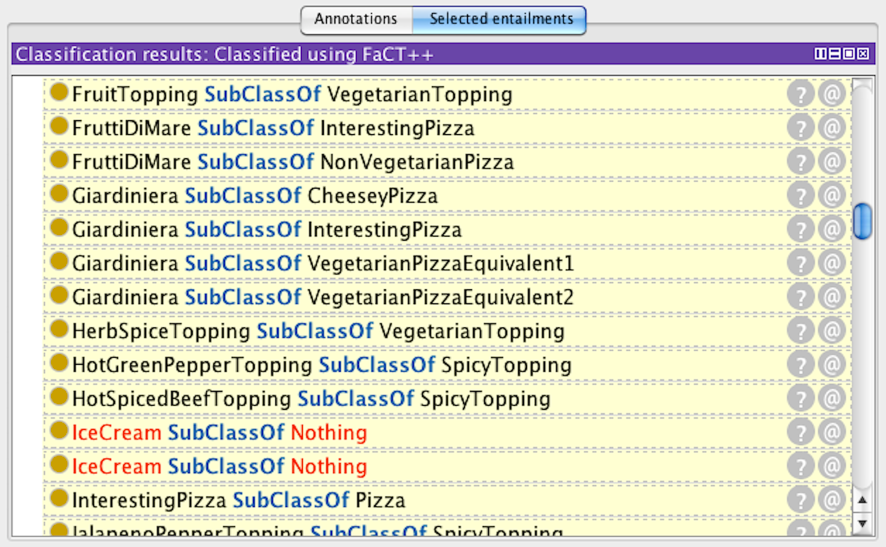
\includegraphics[width=0.9\textwidth]{img/entailment-tab.pdf}
\caption{Screenshot of the \enquote{Selected Entailments} tab in \protege}
\label{fig:selected-entaiments-tab}
\end{figure}


\subsection{Ontology publishing}

Ontologies that are available on the web may be published as \enquote{compiled} versions, which include the ontology and its entailments of some description. The OWL version of the National Cancer Institute (NCI) Thesaurus, for example, \enquote{includes inferred relationships}.\footnote{\url{http://evs.nci.nih.gov/ftp1/NCI\_Thesaurus/ReadMe.txt}} There is, however, no definition of what is regarded as an inferred relationship, how these relationships are determined, and what the selection criteria is. This may leave users wondering what kinds of information they are dealing with, and what implications this has for their understanding of the ontology. 

\subsection{Metrics and analytical applications}
Analytical applications that consider the number and types of entailments in order to infer ontology metrics depend on clearly defined finite entailment sets as the basis of their  measurements, i.e.\ \emph{what exactly} is measured. The entailment set used to generate metrics must be well defined and independent from a particular implementation or \emph{individual modifications} of results provided by the OWL API. From anecdotal evidence we know that developers of analytical tools frequently modify the results of the OWL API's \texttt{InferredAxiomGenerator} for use in their application, for example by removing entailments of the type \dlcn{A \subcls \top}. 

One such application is the use of entailment and justification metrics for the purpose of identifying ontology design styles \cite{mikroyannidi11aa} which ensures transparent and consistent measurements across different applications by clearly specifying the type of entailment set to be extracted. 

Another example is the counting of entailments which are lost in the debugging process of the OWL SafeMode tool \cite{scharrenbach11aa} in order to evaluate the quality of a repair step, which  requires a stable way of counting entailments that is not sensitive to the irregularities discussed above.

Finally, some approaches to ontology \emph{diffs}, that is, determining and quantifying the semantic and syntactic differences between two ontologies (e.g. two versions of an ontology), make heavy use of finite entailment sets. In these approaches the difference between two ontologies is measured based on the (countable) differences in their (finite) entailment sets. Gon\c{c}alves et al.\ \cite{goncalves11xz,Goncalves:2012kx} present several approximations to diffs which are based on increasingly complex types of entailment sets, such as entailed atomic subsumptions, subsumptions between complex class expressions already found in the ontologies, and a \emph{grammar diff} which generates new complex expressions to check for entailment.


\subsection{Imported and native entailments in BioPortal}
In a survey of 42 OWL and OBO ontologies from the NCBO BioPortal \cite{bail11jm}, we found that imported entailments (in the $(AI^{nim})^+$ set of atomic subsumptions of type $A \subcls B$ for satisfiable classes $A, B$) did in fact have a visible effect on the number of entailments found in those ontologies. In this corpus, the upper-level ontology \emph{Basic Formal Ontology (BFO)} \cite{grenon04aa} contributed significantly to the skewing of entailment counts. Table \ref{tab:bfo} shows an overview of the ontologies in the survey.

\begin{table}[htb]
\centering
\caption{Ontologies and imported entailments in the NCBO BioPortal.}\label{tab:bfo}	
\begin{tabu}{ccccccc}
\toprule
& \multicolumn{3}{c}{Importing BFO} & \multicolumn{2}{c}{Other imports} & \\
\cmidrule(r){2-4}\cmidrule(r){5-6}  
Ontologies & Total & Imported & Mixed & Total & Split & No imports \\
\midrule
42 & 7 & 3 & 4 & 7 & 5 & 28\\
\bottomrule
\end{tabu}
\end{table}

7 ontologies in the sample corpus imported BFO, of which 3 had no native entailments at all, but only 70 imported entailments which all originated from BFO. A further 4 ontologies had 70 imported entailments from BFO, plus additional entailments which were either native or imported from ontologies other than BFO. 

Additionally, a further 7 ontologies had imported entailments from ontologies other than BFO; for 5 of these, however, the imports could be attributed to the ontology being intentionally split up over several files with similar file names. Examples of these included the \emph{Chemical Information} ontology \cite{konyk2008aa}, which had 1 native entailment, 72 imported entailments from an ontology titled \enquote{cheminf-external}, and 3 entailments from \enquote{cheminf-core},  or the \emph{Semanticscience Integrated Ontology} (SIO),\footnote{\url{http://code.google.com/p/semanticscience/wiki/SIO}} which had imported entailments from an ontology called \emph{sio-core.owl}. 

Finally, 28 ontologies did not have any imported entailments at all, which could be either due to them having no imports, the imported ontology having no entailments that matched our criteria, or missing imports, which were ignored in the pre-processing stage when downloading the ontologies from BioPortal.

The example of the BioPortal ontologies shows how an analysis or comparison of ontologies based on the number of entailments and justifications needs to pay attention to their import structure; in the case of the BFO imports, the 3 ontologies which had only entailments from BFO would have appeared to have exactly the same number of entailments and justifications,  and thus might have been wrongfully classified as similar in terms of their expressivity and inferential power.


\section{Summary and conclusions}

In this chapter, we presented a discussion of the issues surrounding finite entailments sets for OWL ontologies. While the classification and computation of inferences is a standard reasoning task in the ontology engineering process, there exist ambiguities in ontology tools as to what constitutes the \enquote{set of entailments} of an ontology. We highlighted various design decisions to be made in order to clearly specify a non-ambiguous finite entailment set of an OWL ontology: how to deal with tautologies, whether to include asserted axioms, how to deal with transitive and non-strict subsumptions, and how to make the transition from nodes and edges in an abstract class graph to concrete sets of \emph{axioms} which are presented to a user or used in an OWL application. We also highlighted the problem of \emph{imported entailments} and how these can skew ontology metrics based on entailments, which was demonstrated using examples from a corpus of biomedical ontologies. The examples found in this chapter illustrate the wide scope of different entailment sets that can be specified depending on the application, ranging from minimal representations which are  suitable for user-facing applications, to exhaustive, yet finite, sets which may be used for analytical purposes.

The outcome of the work presented in this chapter is a deeper insight into what we mean by the \enquote{set of entailments} of an ontology, alongside a set of properties which can be used to precisely define a finite entailment set that is fit for a specific purpose. The main benefit of this set of properties is that it is defined from an \emph{application} perspective, which makes the effects of individual choices, such as whether to include indirect subsumptions, easier to understand for a user. Finally, we have made available a prototypical entailment generator on top of the OWL API, which allows the straightforward specification of finite entailment sets using a custom configuration file. The understanding and tools gained here lay the foundations for our discussion of the relations between justifications for entailment sets, which will be presented in the following two chapters.

